\section{Methods}
\label{sec:methods}
\begin{figure}[tb]
  \begin{center}
    \begin{tabular}{ccc}
    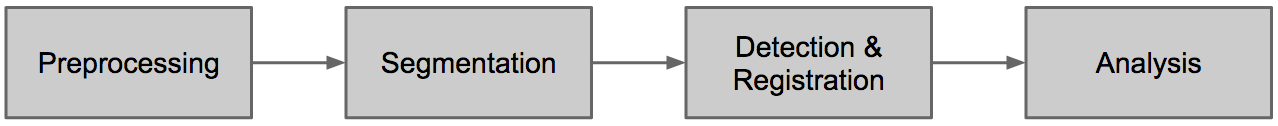
\includegraphics[width=\figfullwidth] {fig/framework.png}
    \end{tabular}
    \caption{ \label{fig:framework} Illustration of the proposed 4D CT image processing framework. From CT image preprocessing, image segmentation, landmark detection and functional data registration, to final analysis.
    }
  \end{center}
\end{figure}

% How do I approach it?
To perform data analysis for subjects with large spatial differences, spatial normalization in the form of registration is an important step.
Registration can be approached in different ways.
First, image registration, which uses image intensities as features, has been developed in medical image analysis for the past decade.
Most of these methods have to do with defining an energy function with data term (dissimilarity between source image and target image) and regularization term (atypicality of mapping from source image to target image),
and then develop optimization method to find a best mapping which minimizes such energy.
See the review articles by Hill et al. and Sotiras et al. on this topic~\cite{hill2001medical,otiras2013deformable} for details.
For particular application for registration on one subject among a short time period, Guerrero et al. developed a deformable algorithm for dynamic ventilation imaging from 4D CT~\cite{guerrero2006dynamic}.

On the other hand, shape registration, which uses geometric cues as major features, has succeeded in many applications in computer vision and computer graphics~\cite{belongie2002shape,li2012temporally}.
With the same fashion of energy minimization framework as image registration, these methods rely on shape features, e.g. curvature or level of bending, to define the data term.
However, using such techniques to align pediatric airway data is still difficult.
Hong et al. proposed a simplified airway model which allows for much easier registration for further analysis~\cite{hong2014statistical}.
Figure~\ref{fig:Fleck} shows the anatomy I am looking at in this work.
I started this project by extending Hong et al.'s simplified airway model to a 4D CT processing framework.
Figure~\ref{fig:framework} illustrated the automatic 4D CT processing framework.


% Need to familiar with
\subsection{Image preprocessing and segmentation}
\label{sec:image_preprocessing_and_segmentation}
The algorithm segmented the airway from 3D CT image using Otsu's method and two manually chosen seeds that bracket the airway.
For better adaptive to current medical image processing libraries, the framework starts with reformatting data from DICOM images to NRRD images.
Then a padding and filtering operator for making the image boundary has the same intensity as air is applied on NRRD images.
With scripts automatically applying preprocessing programs reduced costs of manually operating medical image softwares, such as Slicer or ParaView.

Otsu's method finds a threshold to separate data into two clusters, so as to try to make each cluster as tight as possible.
This is achieved by maximizing the inter-subject variances and minimizing intra-subject variances in terms of voxel intensity.
In our case for segmenting airway, the two clusters were air and non-air regions.
To remove the air regions that were not in the airway, morphological operator closing (with a sphere structuring pattern) first be applied to remove the actual airway.
This computed a map of air regions outside the subject.
We can apply the map as a filter to remove the air outside the airway to get a clean airway in the subject.
Then, two seeds further help to extract trachea and exclude bronchus in the airway.

With this segmentation, the airway can be approximated by statistical models~\cite{pizer2013nested}.
Focus on measuring the size of airway, we used a centerline with cross sections to represent the airway.
The centerline is inferred based on the heat distribution along the airway flow that is solved for by a Laplace equation.
Cross sections are cut from segmented airway geometry using planes that are orthogonal to the centerline. 
The area of the cross sections along the airway is then used as a 1D functional data representation of an airway.

\subsection{Landmark detection}
\label{sec:landmark_detection}
\begin{figure}[tb]
  \begin{center}
    \begin{tabular}{ccc}
    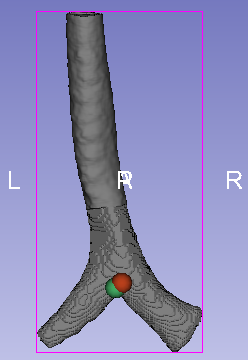
\includegraphics[height=\figheight] {fig/Fleck_005_geometry.png}
    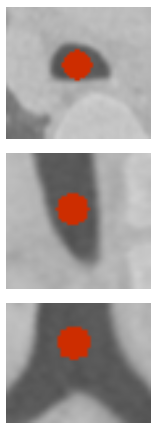
\includegraphics[height=\figheight] {fig/landmark.png}
    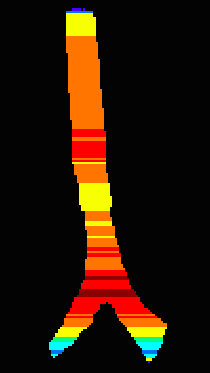
\includegraphics[height=\figheight] {fig/Fleck_005_likelihood.png}
    \end{tabular}
    \caption{ \label{fig:detection} Visualization of the framework of landmark detection. {\bf Left.} First, an airway geometry is segmented by Otsu-thresholding. Green marker is the ground truth annotation and red marker is the predicted location of TC. {\bf Middle.} Second, CHOG features are computed in the center of the trachea in each location along the airway. From top to down: the Axial, sagittal, and coronal plane. {\bf Right.} Finally, visualization of the probabilities of applying the trained classifier on these different hypotheses. Dark red indicates the highest likelihood of TC. In this case, the predicted TC is only 1.97 mm (the total length of the airway is 159 mm) away from the ground truth annotation. This error is only 1.2$\%$ of the entire airway.
    }
  \end{center}
\end{figure}

We can register functional data using some common landmarks across subjects.
Typically landmarks are determined manually.
To reduce the manual annotation cost, based on Dalal and Triggs's object detection framework~\cite{dalal2005histograms}, I propose a landmark detection framework using concatenated Histogram of Gaussian (CHOG) features and a geometric prior. 
Figure~\ref{fig:detection} illustrates the detection of the trachea carina (TC).
The goal of the landmark detection is to capture the dynamics of landmarks.
Therefore, the accuracy of landmark detection should be high enough to compensate the dynamics in the 4D CT image.
If the prediction error is larger than the actual dynamics in the 4D CT image, then the predicted location cannot be determined.

HOG is well designed normalized local histograms of image gradient orientation in a dense sample grid.
The original purpose of this feature was for human detection~\cite{dalal2005histograms}.
Given the popularity of HOG based object detectors, researchers even tried to answer why it works (or did not work) by visualizing the feature spaces~\cite{vondrick2013hoggles}.
However, it has more general applicability as it captures edge or gradient structures that are very characteristic of local shape. 
It can also be efficiently computed.
In practice the HOG is implemented by dividing an image window into small spatial cells, for each cell accumulating a histogram of gradient directions with different bins over pixels of the cell.
The concatenated histogram over cells would be the final representation of an image window. 
To apply HOG on 3D images, instead of computing histograms in arbitrary 3D orientations, I computed 2D HOG in the axial, coronal, and sagittal planes, which are the three perspectives for user annotations, and concatenated them together as a three times longer concatenated histogram (CHOG).
In this work, I used this simple trick to generalize HOG from 2D to 3D.

The first step of the landmark detection framework then is to train a binary classifier using CHOG.
For doing high dimensional data and low sample size statical analysis, Distance Weighted Discrimination can be applied to improve the training~\cite{marron2007distance}.
Yet, for simplistic and speed, linear Support Vector Machine (SVM) is used as a baseline throughout study.
In the prediction stage, the trained classifier can then be applied to the detect the particular landmark.
Higher score generally implies a higher likelihood of a hypothesis.

After landmarks are located, I registered the functional data using b-spline curve registration~\cite{ramsay2006functional}.
The technique needs at least four landmarks for registration.
In Hong et al.'s original paper, each subject had five visible landmarks: from nasal spine, choana, epiglottis tip, true vocal cord (TVC), and TC.
In our dynamic data, most of subjects only have TVC and TC due to a limited of view.
So we can only align these curves by fixing the start and the end of the curve and apply linear interpolation.
In some cases, TC is even the only available landmark which makes alignment impossible using linear interpolation.
I therefore apply a heuristic assumption to these special cases.
Given we have decent amount of data,
the assumption is that a given subject has the same length of trachea from TVC to TC as the most relevant subject (in terms of age) in our dataset.
Therefore, we can compute the proportion of the imaged trachea by measuring the ratio of the length of the current trachea in physical space and the length of the most relevant subject from TVC to TC.

\subsection{Statistical atlas analysis}
\label{sec:statical_atlas_analysis}
Given spatially aligned functional data I would like to capture population changes with respect to some factors, say age.
We can use a blending kernel applying on the dataset to interpret a subject with the target age.
For example, I used a Gaussian weight function $w_i(a_i; \sigma, \bar{a}) = c\exp{(a_i-\bar{a})/2\sigma^2}$, where $a_i$ is the age for the observation $i$, $\sigma$ is a predefined standard deviation and $c$ is the normalization constant for fitting data to a specific age.

To further analyze the weighted data, I applied weighted functional boxplots to build a statistical atlas for each dynamic subject~\cite{hong2013weighted}.
Functional boxplots were originally proposed by Sun and Genton~\cite{sun2011functional} based on the definition of band depth for functional data.

Band depth is used to rank functional data for ordering it from the center outward.
To order functional data, we first define a subset and the membership of a data in the subset.
Given a functional dataset, any two function curves in the dataset can form a set in which the region between these two curves belong.
A curve fully belongs in this subset if it is in the region from the beginning to the end of the function.
A curve might be partially belong in the subset.
Figure~\ref{fig:vis_fbplot} shows the difference.
A band depth of a functional data curve can be defined as the ratio of the number of subset in which data fully belongs over all possible subsets.

\begin{figure}[tb]
  \begin{center}
    \begin{tabular}{ccc}
    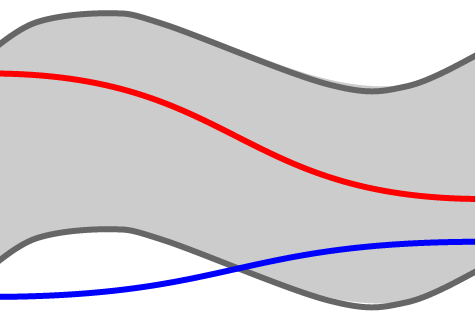
\includegraphics[height=35mm] {fig/illustration_fbplots.png}
    \end{tabular}
    \caption{ \label{fig:vis_fbplot} Visualization of the band depth. The red curve fully belongs to the shaded region, but the blue curve is partially belonged to the shaded region.
    }
  \end{center}
\end{figure}

Given a set of functional data $Y=\{y_i | i=1,...,n\}$, a combinatorial function $C$ which enumerates all two pair combinations in a set, and a band function $B(y_1, y_2) = \{(t,x(t)): t\in \mathrm{T}, \mathrm{min}(y_1(t),y_2(t)) \leq x(t) \leq \mathrm{max}(y_1(t),y_2(t))\}$,
the band depth $D$ of a functional data $y$ with respect to a set $Y$ can be defined as

\begin{equation}
D(y; Y) = \sum_{y_i, y_j \in C(Y)} I[y \subset B(y_i, y_j)],
\label{eq:band_depth}
\end{equation}
where $I$ is an indicator function.
A generalized version of band depth is the weighted modified band depth

\begin{equation}
D'(y; Y) = \sum_{y_i, y_j \in C(Y)} w_iw_j\lambda[ B(y_i, y_j) ]
\label{eq:weighted_band_depth}
\end{equation}
where $\lambda$ is the Lebesgue measure, and $w$s are the weights of data for fitting the population.
If a curve $y$ is only partially in a subset $B(y_i,y_j)$, the $\lambda$ measures the ratio of time that $y$ is in the subset $B(y_i,y_j)$.
If a curve is fully in the subset, the $\lambda$ measurement is one.
I applied (\ref{eq:weighted_band_depth}) to compute a population atlas and to plot subject dynamics upon the population atlas using (\ref{eq:band_depth}).

When a rank of functional data is available, we can compute interesting statistics such as median, interquartile range, and outliers of the population.
For example, given a set of dynamic data $S$ and a normal control atlas $N$, to identify an abnormal airway collapse, we can apply point estimator on the functional data that is out of the normal control atlas.
The maximum ``Collapsed dynamics'' can be defined as
\begin{equation}
% E(S, N) = \frac{\max_i(s_i)-\min_i(s_i)}{\max_i(s_i)}, \forall i, j s^j_i \in S < \inf N_i.
E(S, N) = \frac{\max_x(s_x)-\min_x(s_x)}{\max_x(s_x)},
\label{eq:collapsed_dynamics}
\end{equation}
where $x=\{i, s_i < n_i | s \in S, n = \inf N \}$